% \lipsum[4] Citing \cite{InfH} properly.
% Was ist eine \gls{guid}?
% Eine \gls{guid} kollidiert nicht gerne.

% Kabellose Technologien sind in abgelegenen Gebieten wichtig \cite{APCW2006}.
\setauthor{Martin Hausleitner}
% 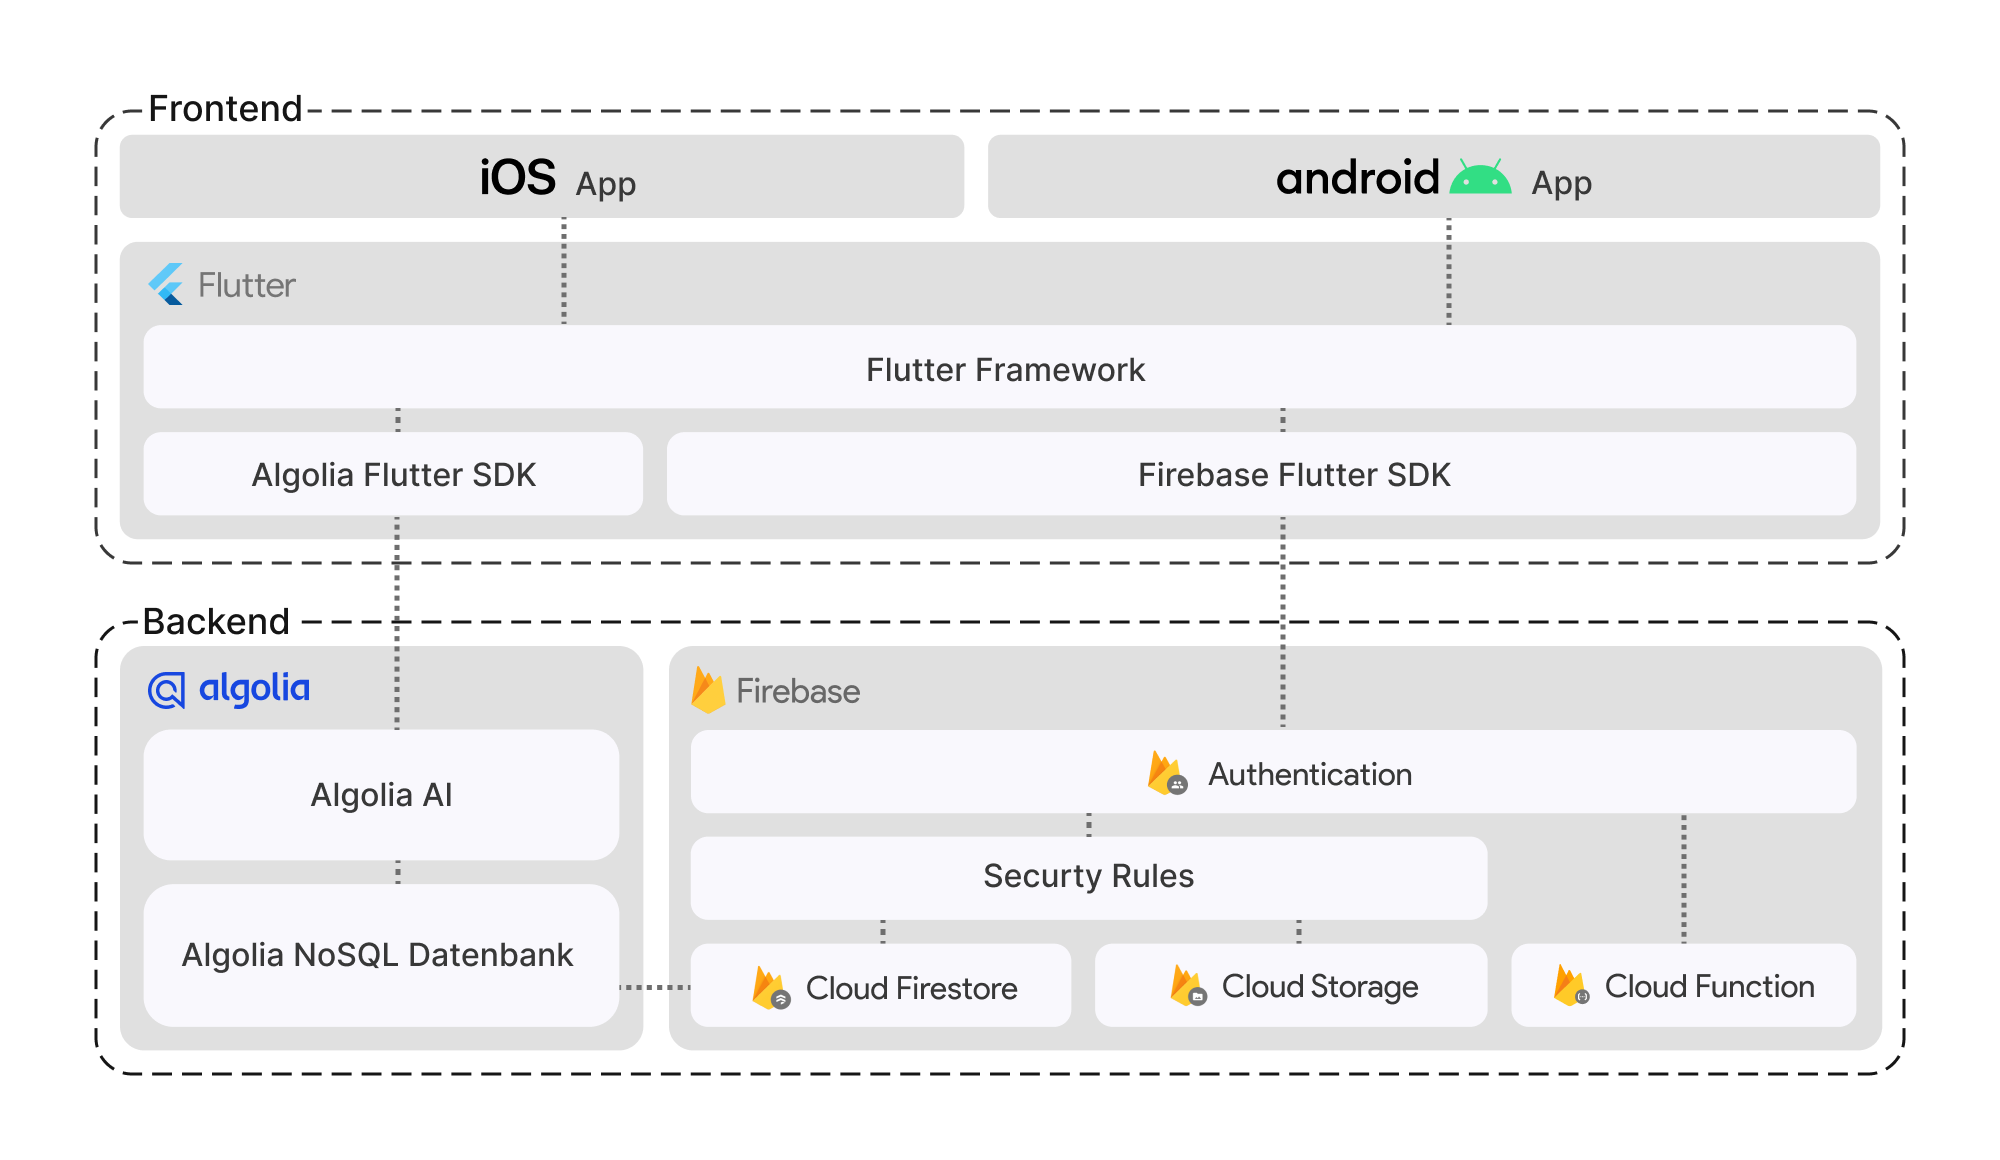
\includegraphics[width=0.2\textwidth]{pics/systemarchitektur_diagram.png}
\begin{figure}[h]
    \centering
    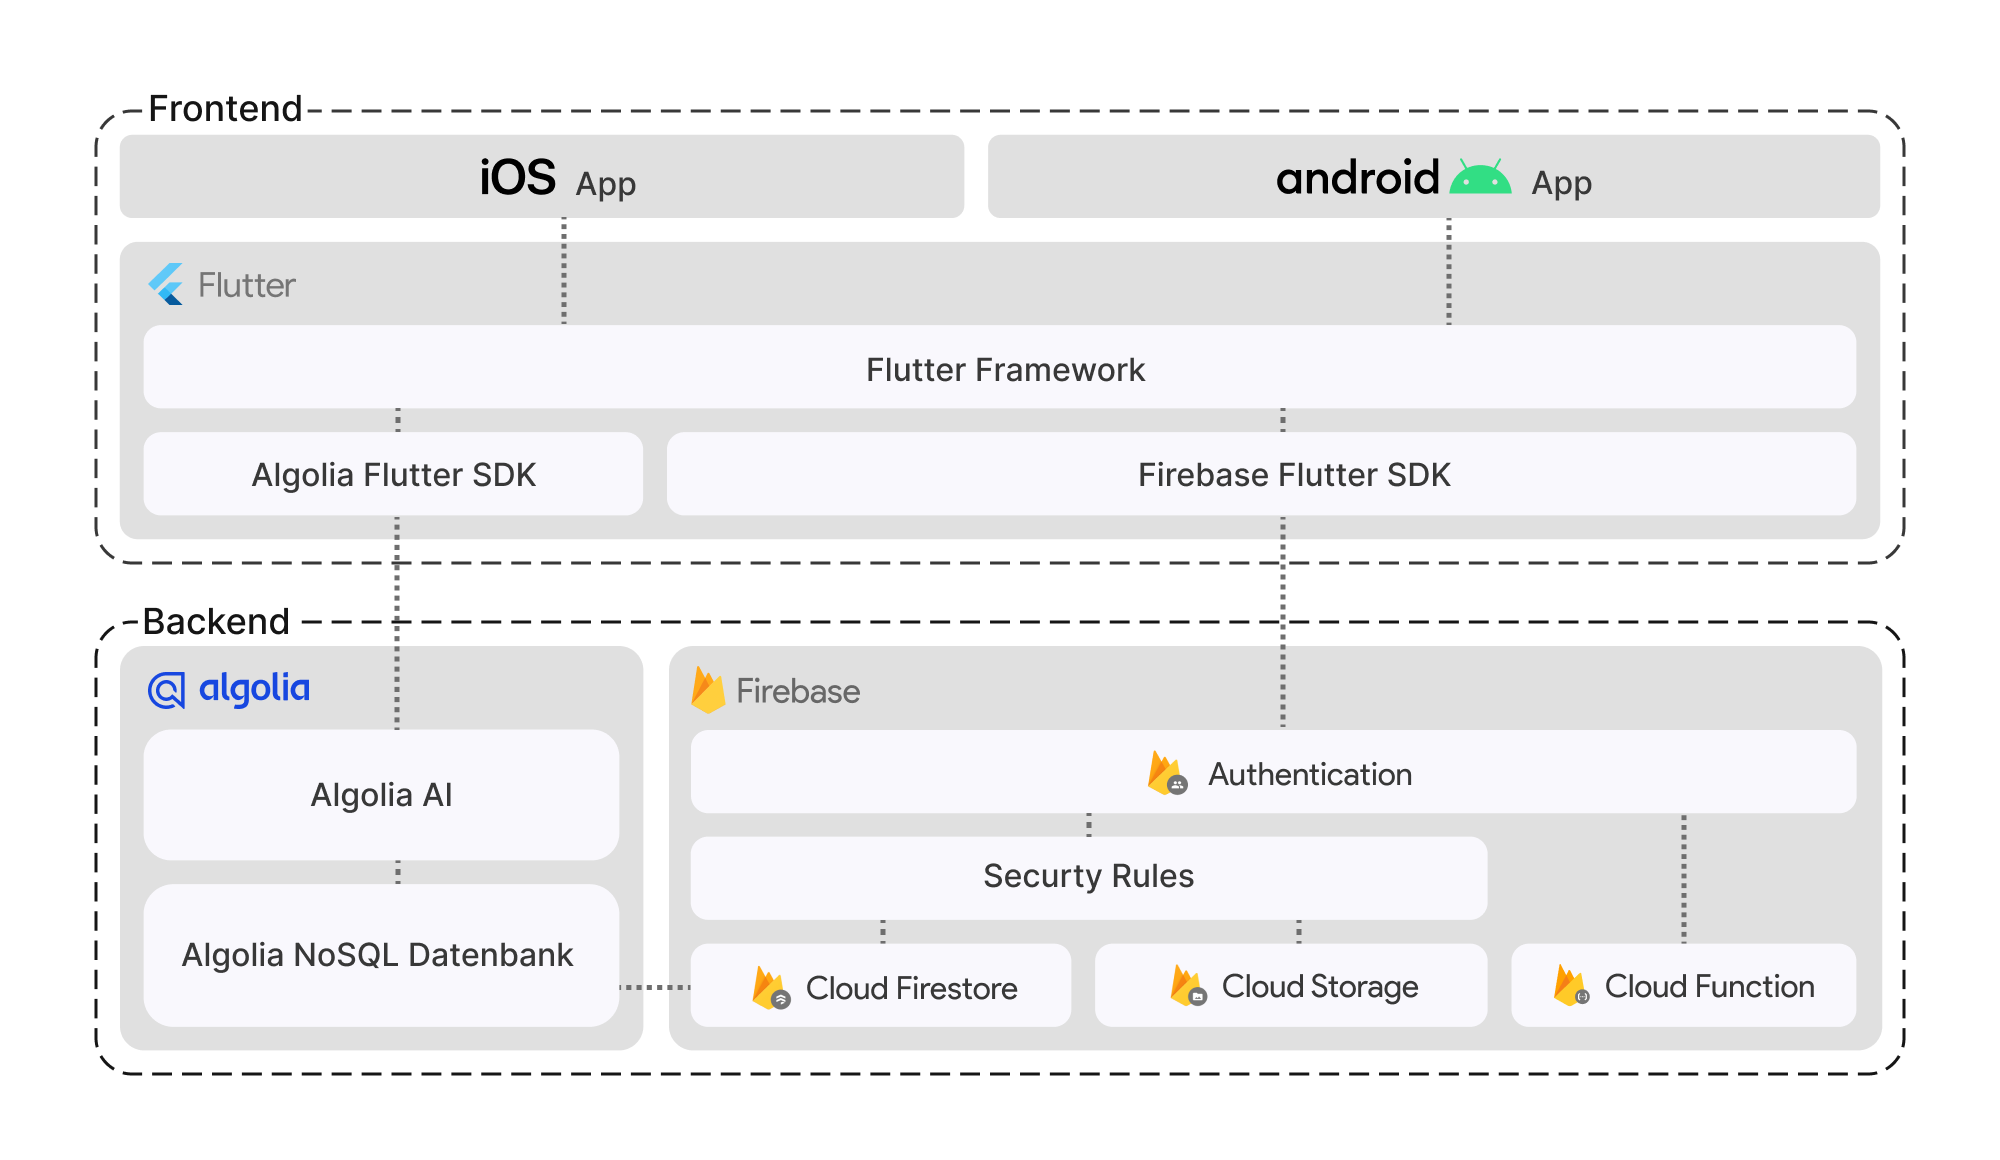
\includegraphics[width=1\textwidth]{pics/systemarchitektur_diagram.png}
    \caption{Systemarchitektur Diagramm}
    \label{fig:systemarchitektur}
    \end{figure}
% todo: add systemarchitektur_diagram
% 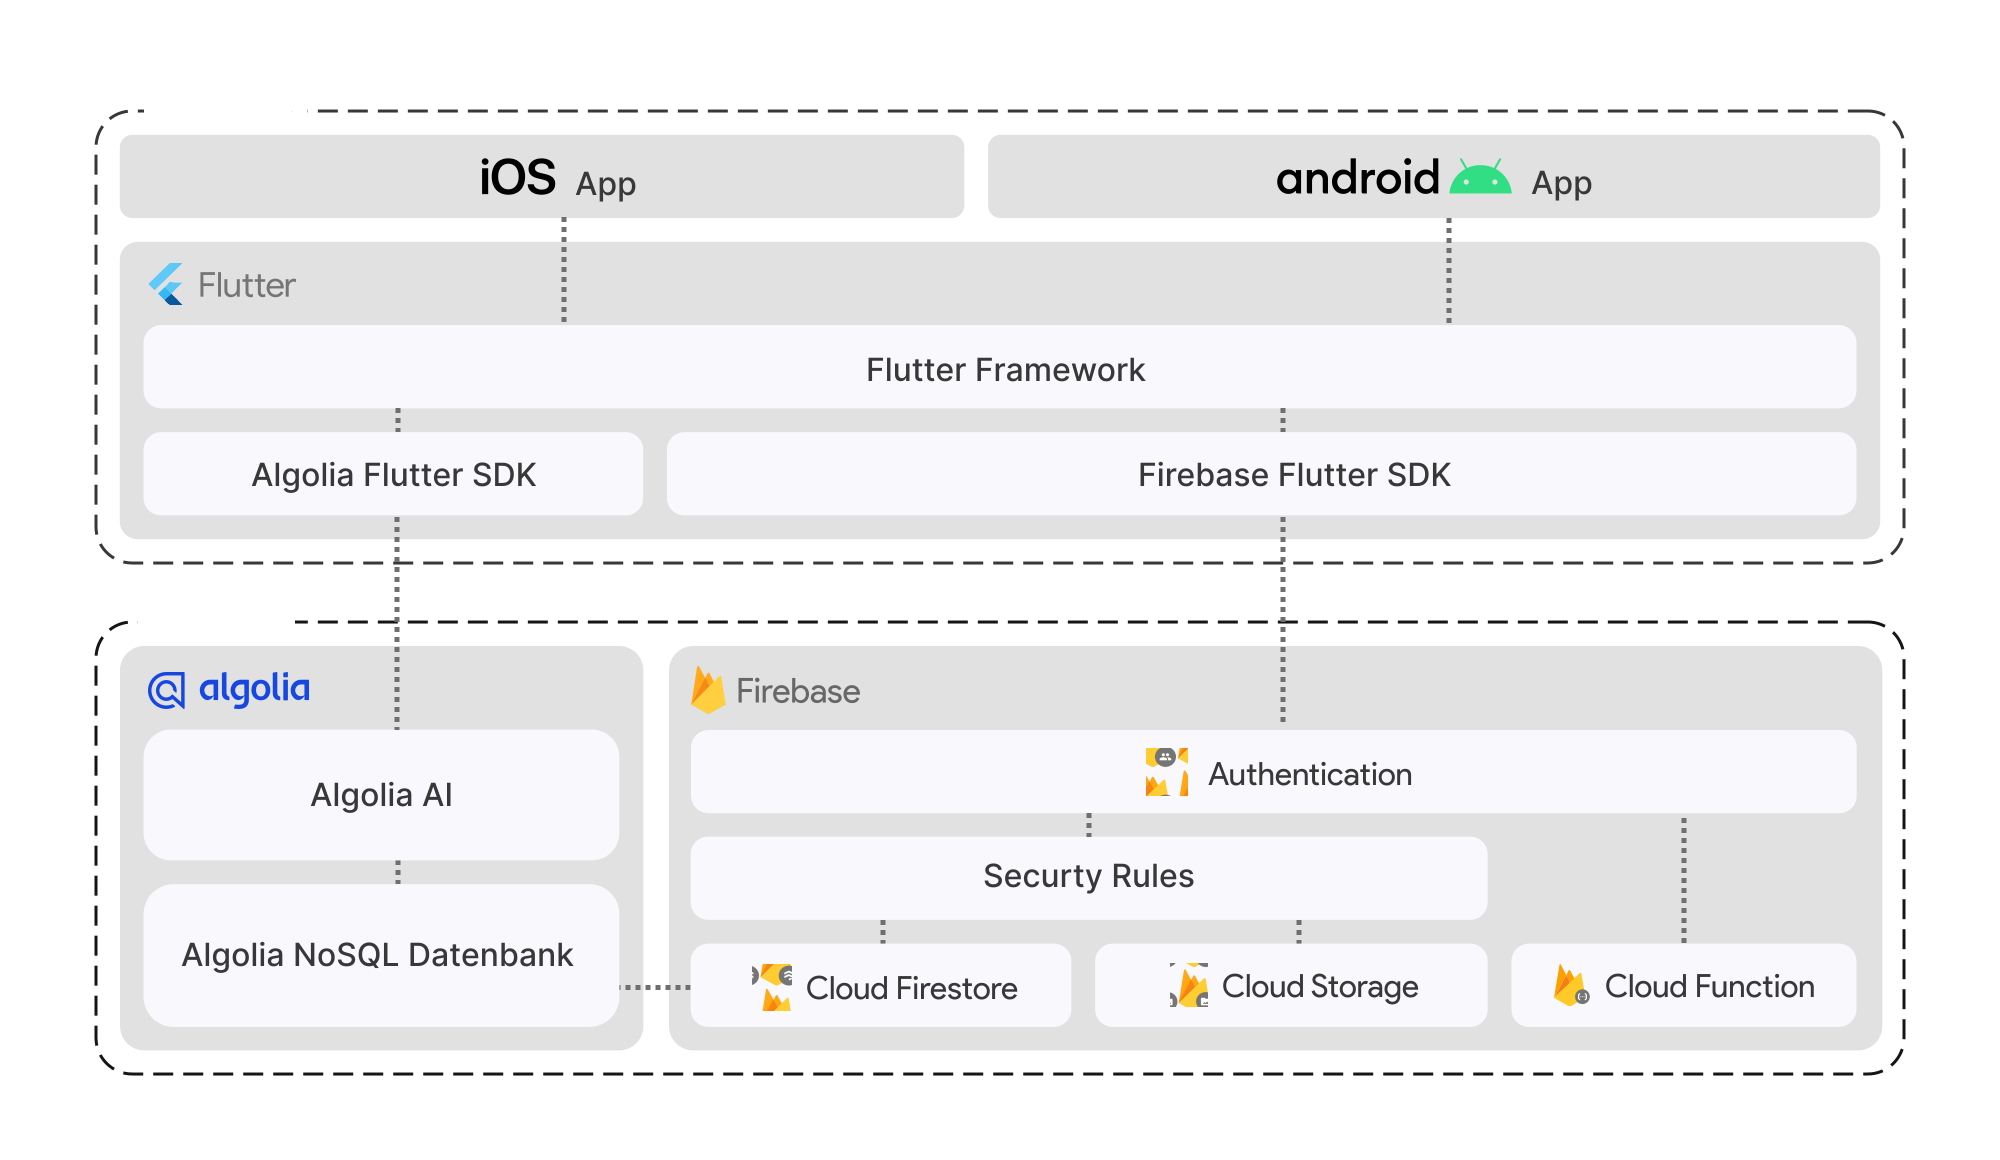
\includegraphics[width=0.2\textwidth]{pics/systemarchitektur_diagram.svg}

% \includesvg{pics/systemarchitektur_diagram.svg}
Die vorliegende Abbildung \ref{fig:systemarchitektur}
veranschaulicht vereinfacht unsere Systemarchitektur. Der
obere Teil stellt das Frontend dar, welches vollständig im
Flutter Framework unter Verwendung der Programmiersprache
Dart entwickelt wurde. Zur Kommunikation mit dem Backend
wurden die \href{https://pub.dev/packages/algolia}{Algolia
Flutter SDK} und
\href{https://pub.dev/packages/firebase}{Firebase Flutter
SDK} genutzt. Zur Vereinfachung wurden die Funktionen der
Firebase Flutter SDK in einem einzigen Paket
zusammengefasst, während Firebase für jedes Feature ein
eigenes Package bereitstellt. Die Flutter-App wird
anschließend für iOS und Android kompiliert.

Im Backend wurde besonderer Wert auf die Implementierung von
Sicherheitsmaßnahmen gelegt. Der erste Sicherheitslayer ist
die
\href{https://firebase.google.com/docs/auth}{Firebase-Authentifizierung},
die das gesamte Authentifizierungssystem für den Zugriff auf
das Backend regelt. Firebase Cloud Functions können nur von
einem registrierten Account ausgeführt werden. Besondere
Cloud Functions verlangen darüber hinaus eine zusätzliche
Verifizierung der Adresse des Nutzers.

Wir nutzen \href{https://firebase.google.com/docs/firestore}{Firestore}, eine NoSQL-Datenbank von Firebase, um unsere Daten zu speichern. Um auf die Firestore-Datenbank und den \href{https://firebase.google.com/docs/storage}{Cloud Storage} zugreifen zu können, müssen zuerst die \href{https://firebase.google.com/docs/firestore/security/overview}{Firestore Security Rules} durchlaufen werden, die sämtliche Zugriffsrechte auf die Dokumente in der Datenbank oder dem Cloud Storage regeln. Mehr dazu findet sich unter \hyperref[sec:security-rules]{Security Rules}.

Firestore verfügt nicht über eine integrierte Funktion zur
vollständigen Durchsuchung aller Dokumente, weshalb für die
Suche nach Inhalten eine externe Suchmaschine wie Algolia
erforderlich ist. Durch die Verbindung von Cloud Firestore
mit der Algolia SQL-Datenbank wird sichergestellt, dass die
Datenbanken synchronisiert werden. Ein bedeutender Vorteil
dieser Vorgehensweise, der möglicherweise zunächst als
Nachteil betrachtet werden könnte, besteht darin, dass wir
über zwei Datenbanken verfügen, die dieselben Daten
enthalten. Die Algolia-Datenbank verfügt jedoch über eine
integrierte Suchfunktion, die die Suchgeschwindigkeit und
-qualität verbessert, indem nur die Beitrag-Titel,
-Beschreibungen und -Tags gespiegelt werden, anstatt die
gesamte Datenbank zu replizieren. Weitere Informationen zu
Algolia Search ist in dem Abschnitt \ref{sec:algolia} zu finden. 

\section{Flutter}

Hier kommt die Beschreibung der Technologie und deren Vorteile/Nachteile, auf Basis von wissenschaftlichen Studien und Erfahrungen aus der Praxis.

Quellen:

https://docs.flutter.dev/resources/architectural-overview

https://flutter.dev/docs/resources/technical-overview,
https://pub.dev/packages/flutter


% \subsection{iOS}
% \subsubsection{CI/CD}

% \subsection{Android}
% \subsubsection{CI/CD}
% \subsubsection{Firebase App Distribution}




\section{Firebase}
\setauthor{Martin Hausleitner}
Firebase\cite{firebase} ist eine von Google entwickelte Plattform für die Entwicklung von Web- und mobilen Anwendungen. Die Plattform bietet eine Vielzahl von Tools und Diensten, die es Entwicklern ermöglichen, schnell und einfach skalierbare Anwendungen zu erstellen.

Die Systemarchitektur von Firebase basiert auf der Cloud-Computing-Technologie, bei der die Anwendungslogik und Daten in der Cloud gehostet werden. Dies bedeutet, dass Entwickler keine physischen Server oder Infrastrukturen verwalten müssen, um ihre Anwendungen zu betreiben. Stattdessen können sie sich auf die Entwicklung der Anwendungslogik konzentrieren und die Firebase-Plattform übernimmt den Rest.

Firebase bietet auch eine Echtzeit-Datenbank, die es Entwicklern ermöglicht, Daten in Echtzeit zwischen ihren Anwendungen zu synchronisieren. Darüber hinaus bietet Firebase eine Vielzahl von Tools und Diensten, darunter Authentifizierung, Benachrichtigungen, Hosting, Speicherung und vieles mehr.

Dank dieser Systemarchitektur und der bereitgestellten Tools und Dienste können Entwickler mit Firebase schnell und einfach skalierbare Anwendungen erstellen und betreiben.

\subsection{Firebase Authentication}

Beschreibung der Firebase Authentication Technologie, inklusive Sicherheitsregeln und Best Practices.

Quellen:

https://firebase.google.com/docs/auth

https://medium.com/flutter-community/firebase-authentication-in-flutter-752d14209a8a

\subsubsection{Security Rules}\label{sec:security-rules}
\setauthor{Martin Hausleitner}
In unserer App ist die Sicherheit ein sehr wichtiger Faktor,
um die Vertraulichkeit und Integrität der Daten und der
Nutzer zu gewährleisten. Firebase bietet für seine
Cloud-basierten Datenbank- und Speicherlösungen - Cloud
Firestore und Cloud Storage - die sogenannten Security
Rules\cite{firebase-rules-docs}\cite{firestore-rules-firestore-nochba}\cite{storage-rules-storage-nochba}, um den Zugriff auf
die Daten und Ressourcen zu kontrollieren. Diese Regeln
definieren, wer auf welche Art und Weise auf welche Daten
zugreifen darf.

Die Security Rules für Cloud Firestore und Cloud Storage sind in einer eigenen Sprache geschrieben und werden serverseitig auf Firebase-Servern ausgeführt. Die Syntax basiert auf einer ähnlichen Struktur wie JSON und erlaubt komplexe Abfragen. Die Regeln können für eine bestimmte Sammlung oder einen bestimmten Pfad definiert werden und erlauben es, bestimmte Bedingungen für Lese- oder Schreibzugriffe zu definieren.


\begin{lstlisting}[language=Python,caption=Security Rules Beispiel]
    match /posts/{postId} {
        allow read: if request.auth.uid != null;
        allow write: if request.auth.uid == resource.data.author;
      }
\end{lstlisting}

Diese Regel definiert, dass jeder Nutzer Lesezugriff auf
alle Posts hat, aber nur der Autor des Posts ihn auch ändern
darf.

Insgesamt bieten die Security Rules für Cloud Firestore und Cloud Storage eine leistungsstarke und flexible Möglichkeit, die Zugriffsrechte auf die Daten und Ressourcen in einer Firebase-App zu steuern. Mit Hilfe der Security Rules können wir sicherstellen, dass die Daten ihrer Nutzer geschützt und nur von berechtigten Personen abgerufen oder geändert werden können.



\subsection{Cloud Firestore}

Vorstellung der Datenbanktechnologie Firestore

Quellen:

https://firebase.google.com/docs/firestore

https://medium.com/flutter-community/firebase-cloud-firestore-in-flutter-26c6e8c6f90c

\subsubsection{Datenmodel}

Hier kommt die Erklärung des Datenmodells in Firebase Firestore und dessen Auswirkungen auf die App-Architektur.

Quellen:

https://firebase.google.com/docs/firestore/data-model

https://www.raywenderlich.com/6628345-cloud-firestore-for-flutter-getting-started

Weitere wichtige punkte:

\begin{compactitem}
    \item Präsentation des eigenen Datenmodells in der Arbeit.
    \item Diagramme werden verwendet, um das Modell zu präsentieren und Entscheidungen zu erläutern und zu begründen.
    \item Anforderungen der App-Architektur werden dabei berücksichtigt werden.
    \item Performance, Skalierbarkeit und Strukturierung können thematisiert werden.
    \item Zur Veranschaulichung unserer eigenen Datenmodell-Entwicklung kann auf ein Beispiel-Datenmodell-Diagramm auf der offiziellen Firebase-Website verwiesen werden, welches uns als Orientierungshilfe diente.
\end{compactitem}

Beispiel-Datenmodell-Diagramm Quelle:

https://firebase.google.com/docs/firestore/data-model\#structure\_your\_data

\subsection{Cloud Storage}

Beschreibung der Cloud Storage Technologie in Firebase und deren Einsatz in der App.

Quellen:

https://firebase.google.com/docs/storage

https://medium.com/flutter-community/firebase-cloud-storage-in-flutter-flutter-an-firebase-tutorial-c5de7835c6cd

\subsection{Firebase Cloud Functions}
\setauthor{Martin Hausleitner}
Firebase Cloud Functions\cite{firebase-cloud-functions} ermöglichen es uns, unsere Business-Logik wie beispielsweise den Registrierungsprozess und viele andere Logikvorgänge einfach und effektiv in der Cloud abzubilden. Wir haben uns entschieden, die Funktionen in TypeScript zu schreiben, da es uns viele Vorteile bietet, wie zum Beispiel eine statische Typisierung, verbesserte IDE-Unterstützung und eine erhöhte Code-Lesbarkeit.

Der Registrierungsprozess ist ein gutes Beispiel dafür, wie wir Firebase Cloud Functions einsetzen können. Anstatt eine monolithische Anwendung zu erstellen, die alles in einem einzigen Server handhabt, können wir die Logik in kleinere Funktionen aufteilen, die jeweils eine spezifische Aufgabe erfüllen. 

Firebase Cloud Functions bietet viele Vorteile, wie zum Beispiel die Möglichkeit, die Funktionen einfach zu skalieren und automatisch zu verteilen, um hohe Lasten zu bewältigen. Außerdem können wir die Funktionen einfach testen und debuggen, indem wir lokale Emulatoren verwenden, bevor wir sie in der Cloud bereitstellen.

Insgesamt sind Firebase Cloud Functions eine großartige Möglichkeit, um unsere Business-Logik in der Cloud abzubilden und unsere Anwendung zu skalieren und zu verbessern. Durch die Verwendung von TypeScript können wir sicherstellen, dass unser Code sauber und robust bleibt und leicht gewartet werden kann.

\section{Algolia Search}\label{sec:algolia}
\setauthor{Arsham Edalatkhah}
Algolia ist eine Suchtechnologie, die es Entwicklern ermöglicht, relevante und schnelle Suchergebnisse für ihre Anwendungen bereitzustellen. Diese Technologie wurde speziell für moderne Anforderungen im Bereich der Suche entwickelt und bietet Funktionen wie automatisches Vervollständigen, Sortierung nach Relevanz und Suche nach Kategorien.

Die Integration von Algolia in eine App-Architektur ist einfach durchzuführen und benötigt keine langen Zeiträume. Es stellt eine RESTful API zur Verfügung, die direkt von der Anwendung aufgerufen werden kann. Es gibt auch integrierte Lösungen für verschiedene Backend-Systeme wie Firebase, was die Integration noch einfacher macht.

Durch die Verwendung von Algolia kann eine Anwendung schnelle und relevante Suchergebnisse bereitstellen, was das Nutzererlebnis verbessert. Es gibt auch eine Vielzahl von Tools und Funktionen, die Entwicklern bei der Optimierung ihrer Suchergebnisse helfen, um die besten Ergebnisse für ihre Nutzer zu erzielen.

Ein Firebase Algolia-Extension ist eine vorgefertigte Integration zwischen Firebase, einer Backend-as-a-Service-Plattform, und Algolia, einer Search-as-a-Service-Plattform. Durch diese Integration können Entwickler leistungsstarke Suchfunktionen in ihre Firebase-Anwendungen integrieren.

Firebase bietet eine Reihe von Tools und Diensten zur Entwicklung und Hosting von mobilen und Webanwendungen, darunter Authentifizierung, Echtzeitdatenbank, Cloud-Speicherung, Hosting und mehr. Algolia hingegen bietet eine leistungsstarke Suchmaschine, die in Echtzeit nach großen Datenmengen suchen kann, sowie Funktionen wie Tippfehler-Toleranz, Autocomplete und Relevanzanpassung.

Als ich meine Diplomarbeit schrieb, habe ich mich für Algolia entschieden, weil es eine leistungsstarke und benutzerfreundliche Suchmaschine bietet, die einfach zu integrieren ist. Algolia ermöglicht es Entwicklern, schnell eine leistungsstarke Sucherfahrung für ihre Benutzer aufzubauen.

Der Firebase Algolia-Extension ermöglicht es Entwicklern, Daten automatisch aus der Firebase-Datenbank in den Algolia-Index zu synchronisieren, was es ihnen ermöglicht, schnell eine leistungsstarke Sucherfahrung für ihre Benutzer einzurichten. Entwickler können die Indizierungseinstellungen anpassen und das vorgefertigte Such-Widget in ihre Anwendung integrieren. Die Erweiterung integriert auch Firebase-Sicherheitsregeln, um den Zugriff auf Suchergebnisse basierend auf Benutzerauthentifizierung und -autorisation zu steuern.

Algolia bietet verschiedene Preismodelle an, die verschiedenen Anwendungsfällen und Budgets entsprechen. Für kleinere Projekte gibt es einen kostenlosen Plan, der bis zu 10.000 Datensätze und 100.000 Operationen pro Monat bietet. Für größere Projekte bietet Algolia kostenpflichtige Pläne, die mehr Datensätze und Operationen pro Monat sowie zusätzliche Funktionen wie Analytics und Personalisierung bieten.

Kunden können auch zusätzliche Sucheinheiten erwerben, wenn sie die Grenzen ihres Plans überschreiten. Die Kosten für zusätzliche Sucheinheiten variieren je nach Plan und Anzahl der erworbenen Einheiten.

Zusammenfassend basiert die Preisgestaltung von Algolia auf einem nutzungsabhängigen Modell, und Kunden zahlen basierend auf der Anzahl der Suchanfragen und der Komplexität dieser Anfragen, gemessen in Sucheinheiten. Algolia bietet verschiedene Preismodelle an, und Kunden können zusätzliche Sucheinheiten erwerben, wenn sie die Grenzen ihres Plans überschreiten.

Quellen:

•	Firebase: https://firebase.google.com/

•	Algolia: https://www.algolia.com/

•	Firebase Algolia-Erweiterung: https://firebase.google.com/products/extensions/firestore-algolia-search

•	Algolia-Preisgestaltung: https://www.algolia.com/pricing/




Vorstellung der Algolia Search Technologie und deren
Integration in die App-Architektur.

Algolia AI

Quellen:

https://www.algolia.com/doc/

https://www.algolia.com/doc/guides/sending-and-managing-data/send-and-update-your-data/tutorials/firebase-algolia/

\subsubsection{Firebase Cloud Function}

Beschreibung der Firebase Cloud Functions und deren Rolle in der Algolia Integration.

Quellen:

https://firebase.google.com/docs/functions

https://www.algolia.com/doc/guides/sending-and-managing-data/send-and-update-your-data/tutorials/firebase-algolia/
